\documentclass[11pt]{article}

\usepackage[margin=1.1in]{geometry}
\usepackage{amsmath,amssymb,amsthm}
\usepackage{graphicx}
\usepackage{booktabs}
\usepackage[round]{natbib}
\usepackage[colorlinks=true,citecolor=blue,linkcolor=blue,urlcolor=blue]{hyperref}
\usepackage{microtype}
\usepackage{enumitem}

\newtheorem{proposition}{Proposition}
\newtheorem{corollary}{Corollary}
\theoremstyle{definition}
\newtheorem{definition}{Definition}
\theoremstyle{remark}
\newtheorem{remark}{Remark}

\newcommand{\E}{\mathbb{E}}
\newcommand{\Prob}{\mathbb{P}}
\newcommand{\Var}{\mathrm{Var}}
\newcommand{\Hd}{\mathcal{H}_{\delta}}
\newcommand{\ov}{\mathrm{ov}}

\title{When the Treatment Talks Back:\\
Information Limits of Observational Logs from\\
Adaptive Generative Political Communication\thanks{Working paper v0.2
(2026-07-30), prepared for arXiv. Replication code and all numerical results:
project repository (\texttt{when-treatment-talks-back}). All reported numbers
are produced by executed code in the repository; none are placeholders.}}
\author{[Author]\thanks{[Affiliation; contact]. Draft --- comments welcome.}}
\date{July 30, 2026}

\begin{document}
\maketitle

\begin{abstract}
\noindent Large language models now conduct persuasive political conversations
that adapt turn by turn to the human they are persuading. We formalize the
treatment delivered by such a system as a composite object --- a strategy
policy $\pi$, a generation kernel $G$, and an information environment $E$ ---
and define deployment, policy, and turn-level excursion estimands for it. We
then show that conversation logs collected under a deployed policy carry
structurally limited information about turn-level causal effects. First, when
the deployed policy has history-deterministic components, turn-level effects
are nonparametrically unidentified (support failure); in RLHF-tuned
deployments this condition is structurally frequent and design-reinforced.
Second, even with formal positivity, we derive the efficient influence
function for the turn-level excursion estimand and show that its
semiparametric efficiency bound grows exponentially in a \emph{policy
decisiveness} index $D(h) = -\log \min_a \pi(a \mid h)$ --- a functional of
the behaviour policy alone, identified from logs, with the softmax
temperature as one special case. The classical average-treatment-effect
bound is recovered as a degenerate case. We then show that this is not
merely a large constant: along policy sequences whose decisiveness grows
fast enough relative to $n$, a two-point argument gives a minimax lower
bound that is bounded away from zero, so no estimator recovers the
turn-level effect at any rate. Third, the overlap weight mass
concentrates on the policy's learned decision boundary as the policy
sharpens: the surviving estimand is a boundary effect $\beta^{\ov}$ ---
formally a regression-discontinuity estimand at a threshold the policy
learned rather than one the analyst chose --- and we prove this in one
dimension and, via a coarea argument, on a decision manifold in
$\mathbb{R}^d$. We are explicit that this is localization, not stability:
the surviving mass is itself $O(\tau)$. The same argument identifies the deceptively stable-but-biased regime seen
in simulation as two-point indistinguishability rather than estimator
pathology; where estimation becomes \emph{easy} again is a separate
achievability question we leave open. Re-querying
three RLHF-tuned open-weights models on 200 real debate contexts locates
plausible deployments in the difficult region, with the important caveat
that the measured decisiveness is a property of a label projection and is
sensitive to the judge (Section~\ref{sec:study0}). We propose the generative
micro-randomized trial (G-MRT) --- within-conversation turn-level
randomization with a locked evidence bank, gated generation, and
assignment-ITT analysis --- as the design remedy.
\end{abstract}

\section{Introduction}\label{sec:intro}

Conversational AI persuades. In randomized trials, GPT-4 debates shifted
opponents' positions more often than human debaters did
\citep{salvi2025conversational}, and conversations with frontier models moved
policy attitudes with durable effects \citep{hackenburg2025levers}. Yet
measured persuasion effects are small in absolute terms: meta-analytic
evidence from field experiments in political persuasion puts average
effects well under one percentage point \citep{kalla2018minimal}. Small
average effects are what make decomposition --- \emph{which turn-level
behaviors of the AI cause belief change} --- the scientifically and
politically urgent question, since an aggregate near zero is consistent
with offsetting turn-level behaviors of either sign. The strongest
lever in \citet{hackenburg2025levers}, a reward model selecting responses turn
by turn, is precisely the component whose interior remains a black box: it is
an adaptive turn-level policy, and its logs are what an analyst inherits.

This paper asks what those logs can and cannot identify. Our answer is
pessimistic in a precise way and constructive in a precise way.

Pessimistic: the treatment in these systems is not a message but a composite
$(\pi, G, E)$ --- a strategy policy, a generation kernel, and an information
environment. Turn-level contrasts computed from deployment logs face three
distinct failures: (i) support failure where the policy is
history-deterministic (Proposition~\ref{prop:1a}); (ii) an exponential
collapse of the semiparametric efficiency bound in the policy's decisiveness
even when positivity formally holds (Result~A), derived from the efficient
influence function of the excursion estimand itself, with a multi-turn
compounding result under an additional recurrence condition
(Proposition~A-T); and (iii) localization --- the overlap mass that survives
concentrates on the policy's decision boundary, so what remains estimable
longest is a boundary estimand $\beta^{\ov}$, distinct from the population
effect and formally a regression-discontinuity quantity (Result~B and
Corollary~\ref{cor:manifold}). We verify each mechanism in simulation, locate
real deployments on the resulting $(n,\tau)$ phase diagram using re-query
experiments on three RLHF-tuned models, and audit instruction--behavior
slippage in 56{,}831 deployed conversations.

Constructive: each failure corresponds to a specific design element of a
generative micro-randomized trial (G-MRT): uniform turn-level randomization
restores support and overlap; exogenous assignment removes sequential
confounding; regime-defined estimands resolve ill-defined treatments; and a
fidelity protocol with assignment-ITT analysis handles generated-treatment
noncompliance.

Contributions, three and locked: (1) an estimand framework for generative
treatments with a general adaptive action space; (2) temperature-indexed
overlap collapse and localization --- Proposition~\ref{prop:1a}, Result~A
with explicit conditions and an identified decisiveness index,
Proposition~A-T, Result~B proved in one dimension and on a decision manifold
in $\mathbb{R}^d$, the fixed-$\tau$ counterexample, and the $(n,\tau)$ phase
structure; (3) the
G-MRT design with a generated-treatment fidelity protocol. Everything else
--- generator transport, internal-representation methods, simultaneous
inference, constrained policy learning --- is explicitly out of scope
(Section~\ref{sec:discussion}).

\section{Related Work}\label{sec:related}

\paragraph{Texts as treatments, static and sequential.}
\citet{imai2026causal} identify effects of features of generated texts using
internal representations of the generating model. Overlap is not free in that
setting: it is \emph{established}, under a separability condition on the
representation, and the authors are explicit that adjusting naively on
learned representations can destroy it. \citet{nakamura2026dynamic} extend
the framework to \emph{sequences} of treatment features --- including their
position within a text or video --- estimating a marginal structural model
with a jointly learned deconfounder for each feature in the sequence, so the
difficulty that later features depend on earlier ones is squarely within
their scope as well as ours. The distinction we draw is therefore not
``static versus sequential'' but where the loss of overlap originates. In
that line the object is a generated artifact produced by a fixed procedure,
and overlap is a property of the representation the analyst adjusts on. Here
the object is an adaptive policy responding to a human interlocutor, and
overlap is destroyed by the deployed policy's own decisiveness before the
analyst does anything --- which is why our results are bounds on what any
analysis of such logs can achieve, and are complementary to, rather than
competitive with, their estimation framework.

\paragraph{Off-policy evaluation with deficient support.} The
estimation-side face of our problem is studied in the contextual-bandit and
reinforcement-learning literatures: doubly robust off-policy evaluation
\citep{dudik2011doubly,thomas2016data,jiang2016doubly}, and, closest to
Proposition~\ref{prop:1a}, off-policy learning under \emph{deficient
support}, where the logging policy assigns zero or near-zero probability to
some actions \citep{sachdeva2020off}. We draw the boundary in four places.
First, that literature works at the level of specific estimators and their
variance or regret; Results~A--B are statements about the
\emph{semiparametric efficiency bound} --- no regular estimator in the
nonparametric class escapes the rate, which closes the ``use a better
estimator'' escape by construction. Second, we index the collapse by an
interpretable policy parameter (effective temperature of an RLHF-shaped
softmax) and obtain exact boundary geometry in $(n,\tau)$, including a closed
form for the phase boundary in our main design. Third, localization
(Result~B) --- \emph{where} the surviving information lives, and the
$\tau\downarrow 0$ limit of the overlap-weighted estimand --- has, to our
knowledge, no counterpart in that literature, whose remedies (truncation,
regularized weights, support restriction) implicitly change the estimand
without characterizing the limit object. Fourth, our remedy is a
\emph{design} (randomize the turns), not an estimator: the setting is
scientific inference about turn-level persuasion effects, where the analyst
can run an experiment, not a fixed logged dataset to be salvaged.

\paragraph{Micro-randomized trials.} MRTs randomize pre-defined discrete
actions at decision points and target causal excursion effects via WCLS
\citep{qian2022microrandomized,boruvka2018assessing}. We import the excursion
estimand and add what conversation requires: a generation kernel between
assignment and realization, ill-defined observational labels, and fidelity
auditing of generated treatments. LLM-in-MRT precedents exist in
behavior-change messaging; our novelty claim is confined to
within-conversation turn-level randomization of generative political
persuasion with information locking.

\paragraph{Stochastic interventions.} Regime-specific potential outcomes for
stochastic and modified policies
\citep{munoz2012population,kennedy2019nonparametric,young2014identification}
supply our formal object: $\beta$ is defined under a kernel intervention ---
assign the label, realize from $G$. Our addition is the history-dependent
generation kernel and the decisiveness collapse.

\paragraph{Overlap weighting.} $\beta^{\ov}$ connects to overlap weights and
empirical equipoise \citep{li2018balancing}; Result~B gives the
$\tau\downarrow 0$ limit of that estimand under a softmax policy, and
Section~\ref{sec:whynot} argues the limit object is itself policy-relevant.

\paragraph{Information equivalence.} \citet{dafoe2018information} motivate
our separation of form from dose: a persuasive-strategy manipulation that
also changes information content is confounded in exactly the sense our
fidelity audit quantifies.

\paragraph{Support failure is old; its systematicity is new.}
Nonidentification from deterministic treatment assignment is standard since
\citet{robins1986new}. Our claim is not the structure but its origin: RLHF
preference optimization widens score gaps and deployment favors low
temperature, so history-determinism in deployed LLM policies is
\emph{structurally frequent and design-reinforced} --- it cannot be escaped
by collecting better logs from the same deployment.

\section{Generative Treatments}\label{sec:framework}

Individuals $i = 1,\dots,n$ converse over turns $t = 1,\dots,T$. At turn $t$
the system draws an action from its policy, $A_{it} \sim \pi_t(\cdot \mid
H_{it})$, where $H_{it}$ is the interaction history, and realizes an
utterance from its generation kernel, $M_{it} \sim G_\theta(\cdot \mid
A_{it}, H_{it}, E_j)$, where $E_j$ is the information environment (for us: a
locked evidence bank on issue $j$). The user responds $R_{it}$; outcomes
$Y_i$ include belief accuracy, calibration, reactance, and one-week
retention.

\paragraph{The action space is general.} $A_t \in \mathcal{A}$ may be a
discrete strategy label, a continuous generation parameter, or a factorial
cell. As a running example --- and as the implementation object of the
companion experimental paper --- we use a $2\times 2$: form $F \in
\{\text{assertive}, \text{interrogative}\}$ $\times$ dose $D \in
\{\text{high: 4--5 facts}, \text{low: 1--2 facts}\}$.

\paragraph{Treatment is a stochastic intervention.} Potential outcomes are
defined under regimes, $Y_i^{\pi,G}$, with do-notation read as a kernel
intervention: intervene on the label, realize from $G$
\citep{munoz2012population,young2014identification}. Three estimand layers:
\begin{itemize}
\item \textbf{Deployment effect} $\Delta^{\mathrm{dep}} =
\E[Y^{\pi_1,G_1}] - \E[Y^{\pi_0,G_0}]$: what existing RCTs identify.
\item \textbf{Policy effect} $\Delta^{\mathrm{pol}}(G) = \E[Y^{\pi_1,G}] -
\E[Y^{\pi_0,G}]$: holding the generator fixed.
\item \textbf{Turn-level excursion effects} (primary): contrasts of one
turn's action against a pre-specified reference policy $\rho$ (uniform over
$\mathcal{A}$, all $t$, all $h$), with subsequent turns following $\rho$.
Proximal excursions (immediate reactance, belief update) are standard
CEE/WCLS targets \citep{boruvka2018assessing}; distal excursions (final
accuracy, retention) connect to distal causal excursion effect estimation
\citep{qian2025dcee} --- using ordinary WCLS for terminal outcomes is a
known attack point we avoid by construction.
\end{itemize}

\paragraph{Ill-defined treatment in logs.} An observational label
$\tilde{S}_t = s$ corresponds to the realized kernel $M_t \sim G(\cdot \mid
s, H_t)$, a \emph{different distribution at every history}. Label-pooled
contrasts do not correspond to any well-defined treatment pair. Our regime
definition does not ``solve'' this nonidentification; it replaces the
question with a well-posed one --- and the well-posed $\beta$ is identified
only under assignment randomization (Section~\ref{sec:gmrt}).

\section{Why Transcripts Are Not Enough}\label{sec:whynot}

Model the deployed policy's action choice as softmax in a history-dependent
score gap with effective temperature $\tau$: for the two-action case,
$p_\tau(h) = \sigma(\Delta(h)/\tau)$ with $\sigma$ the logistic function.
Deployment practice pushes $\tau$ down; preference optimization pushes
$|\Delta|$ up.

\subsection{Support failure}\label{sec:1a}

\begin{proposition}[Support failure]\label{prop:1a}
If $\pi^{\mathrm{dep}}_t(a \mid h) = 0$ on a positive-probability set of
histories, turn-level excursion effects are nonparametrically unidentified.
\end{proposition}

The counterexample pair requires no latent confounder --- the failure is
support, not confounding. Take $T = 1$, $H \in \{h_0, h_1\}$,
$\pi^{\mathrm{dep}}(1 \mid h_0) = 1/2$, $\pi^{\mathrm{dep}}(1 \mid h_1) = 0$,
$Y(a) \mid H = h \sim N(\mu_a(h), 1)$, and let two DGPs differ only in
$\mu_1(h_1) = c_1$ versus $c_2$. The observed-data law factorizes as
$P(H)\,\pi^{\mathrm{dep}}(A \mid H)\,N(y; \mu_A(H), 1)$, to which the
$(1, h_1)$ stratum contributes nothing; the two DGPs are observationally
identical yet their uniform-reference excursion effects differ by
$P(h_1)(c_2 - c_1)$. The multi-turn version replaces $H$ with
$(X, R_{1:t-1})$ and recovers the time-varying-confounding form. The
structure is \citet{robins1986new}; the LLM-specific claim is frequency and
reinforcement, not inevitability.

\subsection{Exponential collapse of the information bound}\label{sec:resultA}

With $\tau > 0$, positivity holds formally, so the right response to
Proposition~\ref{prop:1a} alone would be ``use IPW.'' Result~A closes that
escape at the level of the efficiency bound.

\begin{proposition}[Result A]\label{prop:a}
Let $D(h) = -\log\min_{a \in \mathcal{A}^*} \pi(a \mid h)$ be the policy's
decisiveness at $h$ (Definition~\ref{def:D}), where $\mathcal{A}^*$ is the
set of actions entering the contrast. Assume (A1$'$) $\Prob\{D(H) \geq d\}
\geq c > 0$; (A2$'$) conditional outcome variances on that set are bounded
below by $\underline{\sigma}^2$; and (A3) the model class is nonparametric in
the outcome regression --- no parametric extrapolation into unobserved
strata. Then the semiparametric efficiency bound for the turn-level
excursion effect satisfies
\[
V \;\geq\; \underline{\sigma}^2\,\rho_{\min}^2\,\E\big[e^{D(H)}\big]
\;\geq\; \underline{\sigma}^2\,\rho_{\min}^2\,c\,e^{d},
\]
with $\rho_{\min}$ the smallest reference probability on $\mathcal{A}^*$.
\end{proposition}

We derive this from the efficient influence function of the excursion
estimand itself (Propositions~\ref{prop:eif} and \ref{prop:aprime},
Appendix~\ref{app:eif}) rather than importing a bound stated for the average
treatment effect. The ATE bound of \citet{hahn1998role} is recovered as the
two-action, degenerate-reference special case. Two consequences are worth
isolating. First, the governing quantity is a property of the behaviour
policy alone and is identified from logs; a softmax at temperature $\tau$
gives $D = |\Delta|/\tau$ as one special case, but the statement covers
truncated and constrained decoding, hard filters, and learned $\arg\max$
rules, none of which are softmax. Second, in a factorial design the relevant
probabilities are the \emph{cell} probabilities, not the marginal for the
factor being contrasted: because the reference regime draws the other factor
from $\rho$, a design in which the form-marginal stays at $1/2$ while cells
become rare still has an exploding bound.

By the convolution theorem, \emph{no regular estimator in the class} attains
lower asymptotic variance: switching from IPW to AIPW recovers no
counterfactual information that the sample does not contain. Parametric
extrapolation escapes the bound, but that is buying identification with an
assumption, and should be said in exactly those words. Effective sample size
is arm-specific Kish: $n_{\mathrm{eff}}(a) = n / \E[1/\pi_\tau(a \mid H)]$.
The slogan ``halving $\tau$ squares the required $n$'' holds within
fixed-gap strata; with heterogeneous gaps the max-gap stratum dominates the
rate.

\begin{remark}[Single-turn bounds are a fortiori multi-turn
bounds]\label{rem:aprime}
Our results are stated for one turn and two actions, while the motivating
setting is a $T$-turn conversation. The gap runs in the harmless direction.
The turn-$t$ excursion estimand conditions on the observed history $H_t$ and
contrasts actions at that turn, with subsequent turns following $\rho$. The
observed-data model factorizes turn by turn; the turn-$t$ factor is exactly
the single-turn problem with propensity $\pi_\tau(\cdot \mid H_t)$, and
identifying $\beta_t$ additionally requires bridging every later turn from
$\pi^{\mathrm{dep}}$ to $\rho$. Discarding the information cost of those
later-turn bridges can only \emph{understate} the difficulty; hence any lower
bound for the single-turn problem at the $(\Delta, \tau)$ prevailing at turn
$t$ is also a lower bound for the conversational problem. ($K$-action
policies reduce to the two-action case via the two arms of the contrast.)
\end{remark}

\begin{proposition}[A-T: multi-turn compounding]\label{prop:at}
Consider the $T$-turn policy value $V(\rho)$ of the uniform reference $\rho$
over $K$ actions, observed under $\pi_\tau$. Start from the semiparametric
efficiency bound for finite-horizon off-policy evaluation with
history-dependent policies \citep{kallus2020double,jiang2016doubly}:
\[
V_{\mathrm{eff}} = \Var(V_1(H_1)) + \sum_{t=1}^{T}
\E_\pi\!\Big[\Big(\textstyle\prod_{s\leq t} w_s\Big)^{2}
\Var(V_{t+1} \mid H_t, A_t)\Big],
\qquad w_s = \frac{\rho(A_s \mid H_s)}{\pi_\tau(A_s \mid H_s)}.
\]
Assume (M1) \emph{uniform recurrence of the high-gap set}: $\Prob(H_{s+1} \in
\Hd \mid h, a) \geq p_\delta > 0$ for every $h \in \Hd$ and every action $a$;
and (M2) a per-turn conditional variance floor $\underline{\sigma}^2$ on
$\Hd$. Then
\[
V_{\mathrm{eff}} \;\geq\; \underline{\sigma}^2 \cdot \Prob(H_1 \in \Hd)
\cdot p_\delta^{\,T-1} \cdot \Big[\frac{e^{\delta/\tau}}{K^{2}}\Big]^{T},
\]
which compounds geometrically in $T$ whenever $\tau <
\delta/\log(K^{2}/p_\delta)$.
\end{proposition}

\begin{proof}[Proof sketch]
All terms of $V_{\mathrm{eff}}$ are nonnegative; keep the terminal one. On
$\Hd$, $\E_\pi[w_t^2 \mid H_t = h] = K^{-2}\sum_a 1/\pi_\tau(a \mid h) \geq
K^{-2} e^{\delta/\tau}$ since the rarest action has probability at most
$e^{-\delta/\tau}$. Induct backward from $t = T$: by the tower property and
(M1) --- whose action-uniformity is what lets the bound pass through each
turn's weight --- each turn contributes a factor $p_\delta\,
e^{\delta/\tau}/K^{2}$, and turn 1 contributes $\Prob(H_1 \in \Hd)\,
e^{\delta/\tau}/K^{2}$. The self-contained derivation of the quoted
efficiency bound is given in Appendix~\ref{app:eif}; our contribution is the
insertion and the induction.
\end{proof}

Substantively, (M1) says decisiveness persists regardless of what the system
does --- as with strongly reactant partisan users. The $K^2$ factor reflects
the conservativeness of the uniform reference and is not optimized; the
excursion version (turn $t$, reference thereafter) follows with exponent
$T-t+1$. The honest reading: more turns make the information limit
exponentially worse, now as a proposition rather than a heuristic.

\begin{proposition}[Minimax collapse]\label{prop:minimax}
Let $M(\pi) := \sup_{d>0} \Prob\{D(H) \geq d\}\,e^{d}$. Consider the model
class in which $\pi$ is known and fixed, $Y \mid A=a, H=h \sim
N(\mu_a(h), \sigma^2)$, and $|\mu| \leq B$. Then for any estimator
$\hat\beta$,
\[
\inf_{\hat\beta}\ \sup_{P}\ \E_P\big|\hat\beta - \beta(P)\big|
\;\geq\; \tfrac14 \min\Big\{\, B\rho_{\min},\ \rho_{\min}\,\sigma
\sqrt{M(\pi)/n} \,\Big\}.
\]
In particular, along a sequence of policies with $M(\pi_n)/n \to \infty$
the minimax risk is bounded away from zero: no estimator recovers $\beta$
at any rate.
\end{proposition}

This is the statement that Proposition~\ref{prop:a} alone does not support.
Proposition~\ref{prop:a} bounds the information constant at a fixed policy,
where $\beta$ remains regularly $\sqrt{n}$-estimable; Proposition
\ref{prop:minimax} says that once decisiveness grows fast enough relative to
sample size, estimability itself fails. The proof (Appendix~\ref{app:eif})
is a two-point argument in which the two laws differ only in the outcome
regression at the rarest action on the high-decisiveness stratum, so that
they are separated in the estimand but nearly indistinguishable in the data.
For the main design $H \sim U(-1,1)$, $M = \tau e^{(1-\tau)/\tau}$ in closed
form, i.e.\ $\log M = 1/\tau - 1 - \log(1/\tau)$.

\emph{The deceptive regime is this indistinguishability.} In the main
simulation design, two laws whose true ATEs differ by $0.198$ --- differing
only in $\beta$ on the rarely-treated region --- are separated by $0.16$
standard deviations of the H\'ajek estimator at $\tau = 0.08$, $n = 2{,}000$,
and still only $0.40$ at $n = 32{,}000$, a sixteenfold increase in sample
size. At $\tau = 0.22$ the same $0.200$ gap is recovered as $0.224$ at
$1.69$ standard deviations. What the phase diagram labels ``biased but
stable'' is not a description of estimator behaviour but an instance of
two-point indistinguishability.

\subsection{Localization, the counterexample, and the phase
diagram}\label{sec:resultB}

\begin{proposition}[Result B, one-dimensional]\label{prop:b}
Let $\omega_\tau(H) = p_\tau(1-p_\tau)$ and $\beta^{\ov}_\tau =
\E[\omega_\tau\{Y(1)-Y(0)\}]/\E[\omega_\tau]$. Assume:
\begin{enumerate}[label=(B\arabic*),leftmargin=3.2em,itemsep=1pt]
\item $H$ has a density $f$, continuous in a neighbourhood of each root;
\item $\Delta \in C^1$ and the root set $\mathcal{R} = \{h : \Delta(h) = 0\}$
      is \emph{finite}, with every root simple ($\Delta'(r) \neq 0$);
\item $c(h) = \E[Y(1)-Y(0) \mid H = h]$ is bounded, and continuous near
      each root;
\item $f(r) > 0$ for at least one $r \in \mathcal{R}$.
\end{enumerate}
together with the tail-separation condition (B2$'$):
$\inf_{\,\mathrm{dist}(h,\mathcal{R}) \geq \epsilon} |\Delta(h)| > 0$ for
every $\epsilon > 0$. Then, as $\tau \downarrow 0$, the normalized overlap
measure $\omega_\tau f / \int \omega_\tau f$ converges weakly to
$\sum_j w_j \delta_{r_j}$ with weights $w_j \propto f(r_j)/|\Delta'(r_j)|$.
In the special case of a \emph{unique} root at $0$ the limit is a single
point mass and
\[
\E[\omega_\tau] = \tau\,\frac{f(0)}{|\Delta'(0)|}\,(1+o(1)),
\qquad
\beta^{\ov}_\tau \to \E[Y(1)-Y(0) \mid H = 0].
\]
\end{proposition}

\begin{corollary}[Decision-manifold localization, $H \in \mathbb{R}^d$]
\label{cor:manifold}
Let $H \in \mathbb{R}^d$ with density $f$, let $\mathcal{B} = \{h :
\Delta(h) = 0\}$, and assume: (C1) $\Delta \in C^1$ and $f$ is bounded and
continuous near $\mathcal{B}$; (C2) $0$ is a \emph{regular value} of
$\Delta$, i.e.\ $\nabla\Delta(h) \neq 0$ on $\mathcal{B}$ --- the
$d$-dimensional analogue of the simple-root condition (B2); (C3)--(C4) the
tail-separation condition of Proposition~\ref{prop:b} holds with
$\mathrm{dist}(\cdot,\mathcal{B})$; and (C5) $0 < \int_{\mathcal{B}}
f/\|\nabla\Delta\| \,d\mathcal{H}^{d-1} < \infty$. Then as $\tau
\downarrow 0$,
\[
\E[\omega_\tau] \;=\; \tau \int_{\mathcal{B}}
\frac{f}{\|\nabla\Delta\|}\,d\mathcal{H}^{d-1}\,(1+o(1)),
\]
and the normalized overlap measure converges weakly to the measure on
$\mathcal{B}$ with $\mathcal{H}^{d-1}$-density proportional to
$f(h)/\|\nabla\Delta(h)\|$. Consequently $\beta^{\ov}_\tau \to
\int_{\mathcal{B}} c\,f/\|\nabla\Delta\| \big/ \int_{\mathcal{B}}
f/\|\nabla\Delta\|$. Proposition~\ref{prop:b} is the case $d=1$, where
$\mathcal{H}^{0}$ is counting measure and $\|\nabla\Delta\| = |\Delta'|$.
\end{corollary}

\begin{remark}[What $\beta^{\ov}$ is]\label{rem:rd}
The limit in Corollary~\ref{cor:manifold} is a boundary estimand in the
regression-discontinuity sense: in one dimension it is exactly $\E[Y(1) -
Y(0) \mid \Delta(H) = 0]$, the conditional effect at the assignment
threshold \citep{hahn2001identification}, and in $d$ dimensions it is the
$f/\|\nabla\Delta\|$-weighted average effect over a boundary, the object
studied in multi-dimensional and geographic RD \citep{keele2015geographic}.
The substantive reading is sharper than an overlap-weighting analogy: logs
from a sharply adaptive system behave less like an observational study than
like a natural experiment at a threshold --- but the threshold is one the
\emph{policy} learned, not one the analyst chose. What is stably estimable
therefore describes the histories on which the policy is \emph{undecided},
which in a decisive deployment is precisely the minority of traffic.
\end{remark}

\begin{remark}[The surviving information also vanishes]\label{rem:bmass}
Proposition~\ref{prop:b} says \emph{where} overlap mass concentrates, not how
much of it there is. Since $\E[\omega_\tau] = O(\tau)$, the effective sample
available for $\beta^{\ov}_\tau$ is itself $O(n\tau)$ and degenerates in the
same limit. Result B should therefore not be read as saying that boundary
information is \emph{stable}: what survives longest is boundary information,
but it too disappears as the policy sharpens. Assumption (B4) is exactly what
prevents the leading term from collapsing to $0 = o(\tau)$; without it the
statement is vacuous.
\end{remark}

\begin{proof}[Proof idea]
$\omega_\tau = K(\Delta(h)/\tau)$ exactly, with $K(u) =
1/[4\cosh^2(u/2)]$ and $\int K = 1$: an approximate-identity kernel. The
tail-separation condition kills contributions away from the roots at rate
$e^{-c(\epsilon)/\tau}$; near a simple root, the change of variables
$v=\Delta(h)$, $v=\tau u$ and dominated convergence give
$\int g\,\omega_\tau f \,dh = \tau\, g(0) f(0)/|\Delta'(0)| + o(\tau)$ for
bounded continuous $g$. Ratios deliver the three claims. With multiple roots,
mass distributes proportionally to $f(r_j)/|\Delta'(r_j)|$. Full proof in
Appendix~\ref{app:resultB}; the multivariate coarea version is
Corollary~\ref{cor:manifold}, proved in Appendix~\ref{app:manifold}.
\end{proof}

\paragraph{Why the boundary estimand matters substantively.} $\beta^{\ov}$
is not a consolation prize; it is the effect in a policy-relevant population.
The decision boundary $\{\Delta(H) = 0\}$ collects the histories at which the
deployed policy is genuinely undecided --- the algorithmic analogue of
clinical equipoise \citep{li2018balancing}. Three consequences. First,
\emph{marginal policy evaluation}: any small change to the policy --- a
regulation, a guardrail, a reward-model update, a temperature change ---
alters behavior precisely on and near this boundary, so the effect among
boundary histories is the first-order term in the value change of any local
policy modification. Second, \emph{auditability}: $\beta^{\ov}$ is the one
turn-level causal quantity a regulator could estimate from logs alone with
stable precision, which makes its scope and its limits worth stating exactly.
Third, the political reading, stated as interpretation rather than result:
histories far from the boundary --- strongly reactant partisan contexts where
the policy is most decisive --- are exactly where population-level causal
information vanishes; what deployment data can tell us about persuasion is
confined to the persuadable margin as \emph{the policy} defines it, not as
the scientist would.

\paragraph{What Result B does \emph{not} say.} At fixed $\tau > 0$, an IPW
estimator with true propensities targets the \emph{population} effect as $n
\to \infty$ --- the estimand does not silently become the boundary effect
because the policy is sharp. Numerically: $\tau = 0.3$, $n = 4\times 10^6$,
$\beta(H) = 1 + |H|$ gives IPW $1.792 \approx$ ATE $1.798 \neq \beta^{\ov} =
1.356$. Formal identification and practical estimability are different
properties; our claims are about the \emph{rate} of information loss and the
\emph{location} of surviving information, never about a change of target.

\paragraph{The joint limit is the real object.} The failure surface lives in
$(n, \tau)$: with $n \gg e^{\delta/\tau}$ the population effect is estimable
(at exploding variance); near $n \sim e^{\delta/\tau}$ variance explodes;
with $n \ll e^{\delta/\tau}$ rare crossover actions never appear in the
sample and estimators become \emph{biased while looking stable} --- the
deceptive regime. Figure~\ref{fig:phase} shows the three regimes for the main
design $H \sim U(-1,1)$, $\Delta(H) = H$, with two \emph{reference} lines.
The dashed line is the Result~A bound with $\delta$ chosen optimally: since
$\Prob(\Hd) = 1-\delta$ here, $\max_\delta (1-\delta)e^{\delta/\tau}$ is
attained at $\delta = 1-\tau$, giving $\log n = 1/\tau - 1 - \log(1/\tau)$.
(Fixing $\delta = 1$, as an earlier version did, puts $\Prob(\Hd) = 0$ and
makes the bound identically zero.) The solid line is the $n_{\mathrm{eff}} =
1$ contour $\log \E[1/p_\tau] = \log(1 + \tau\sinh(1/\tau))$, exact for
this design. We stress that neither line is the observed transition: the
$n_{\mathrm{eff}}=1$ contour is a \emph{necessary} condition, and on a
$13 \times 13$ grid the measured onsets of estimability lie $3$--$5$ nats
above it. Which functional of the decisiveness distribution governs the
transition is open (Section~\ref{sec:discussion}).

\begin{figure}[t]
\centering
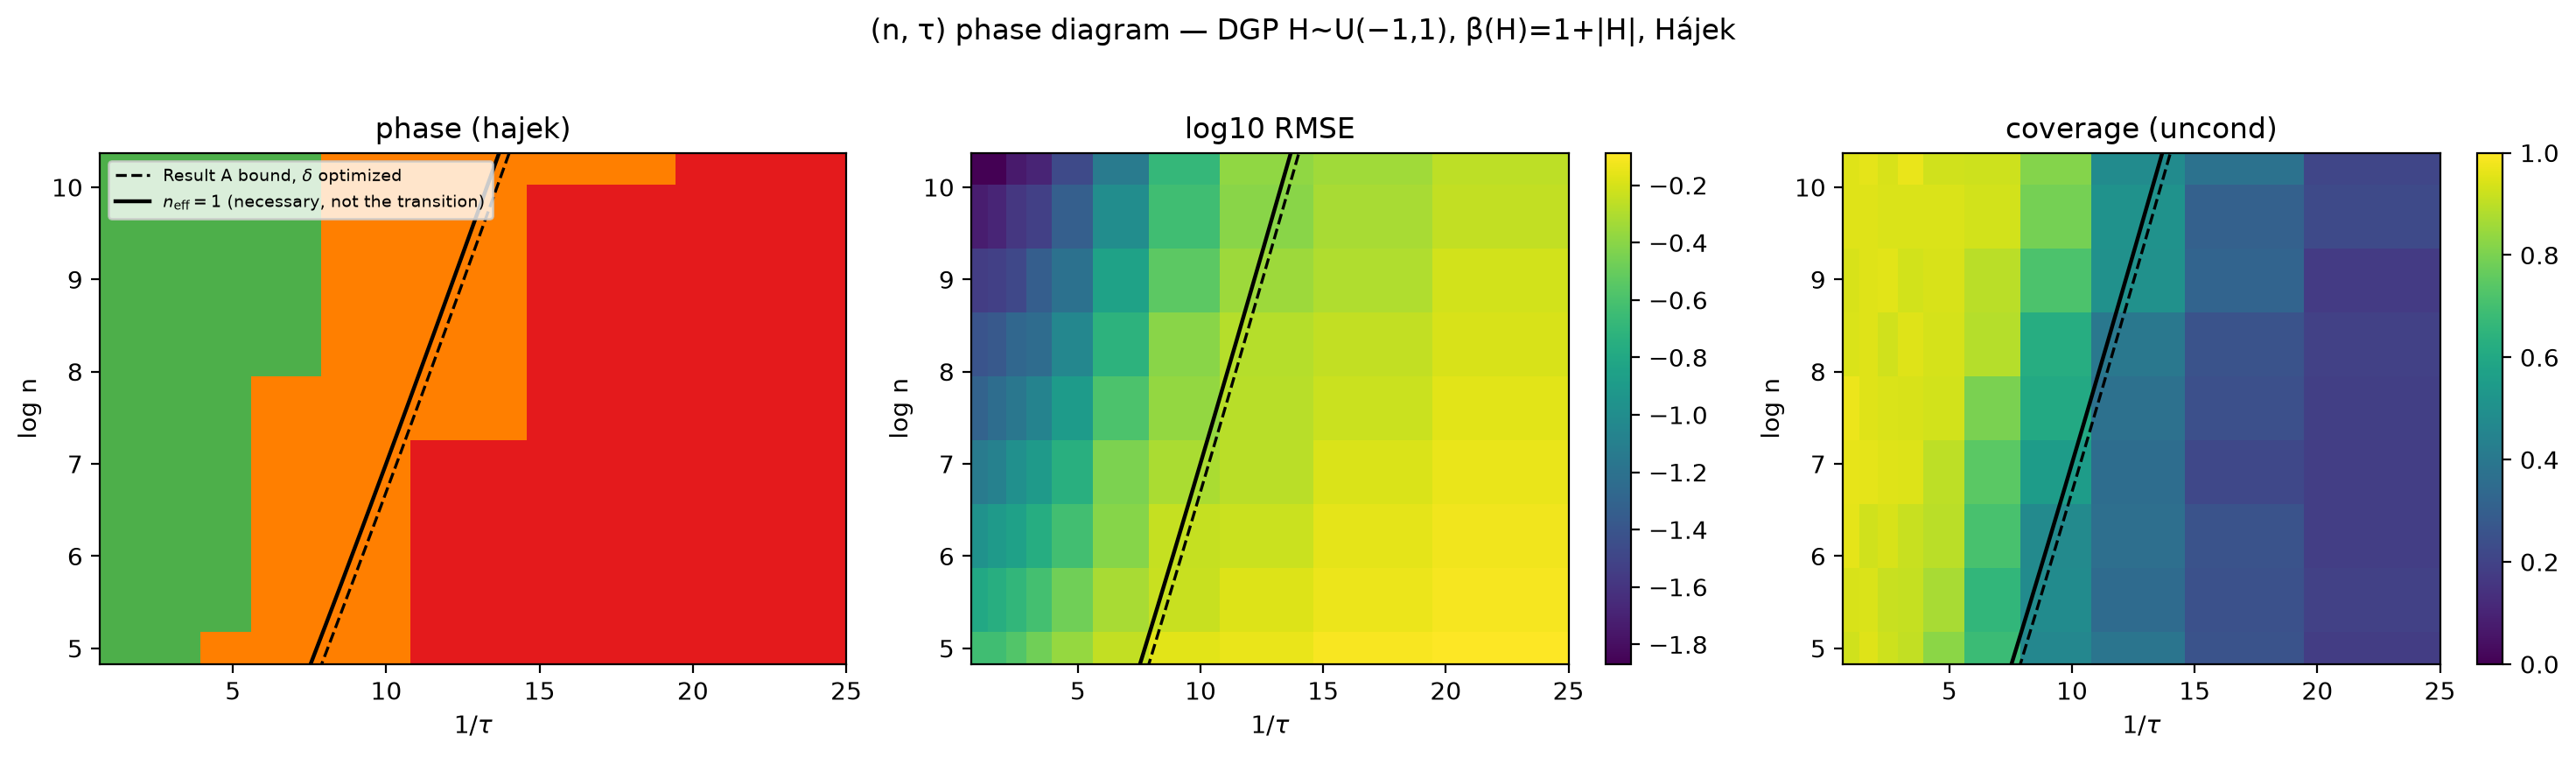
\includegraphics[width=\textwidth]{figs/phase_diagram.png}
\caption{$(n,\tau)$ phase diagram; DGP $H \sim U(-1,1)$, $\beta(H) = 1+|H|$,
H\'ajek estimator, 400 replications per cell. Left: regime classification
(green estimable, orange variance explosion, red biased-stable). Middle,
right: $\log_{10}$ RMSE and unconditional coverage. Dashed line: fixed-gap
heuristic $\log n = \delta/\tau$. Solid line: exact boundary $\log n = \log
\E[1/p_\tau] = \log(1+\tau\sinh(1/\tau))$. Regime thresholds (relative bias
0.10/0.20, coverage 0.85) are presentation choices defended by the RMSE and
coverage panels.}
\label{fig:phase}
\end{figure}

\subsection{Where real deployments sit: Study 0 (descriptive,
motivating)}\label{sec:study0}

Three empirical bridges locate deployed systems on the diagram. Their
epistemic status is \emph{motivating}: they estimate proxies of policy
decisiveness and instruction--behavior slippage, not the parameters of
Sections~\ref{sec:1a}--\ref{sec:resultB}.

\paragraph{(0-a) Reproduction.} Our pipeline reproduces the direction of
\citet{salvi2025conversational} on the released data ($n = 750$):
personalized Human-AI has the largest crude odds ratio for increased
agreement ($2.18 > 1$), matching the original ordering.

\paragraph{(0-b) Re-query decisiveness.} For 200 rebuttal contexts stratified
by treatment and prior-agreement strength, we regenerate $k = 20$ responses
per context and classify the persuasion strategy of each. Across three
RLHF-tuned open-weights families the per-context strategy distribution is
near-degenerate (Table~\ref{tab:models}).

\begin{table}[t]
\centering
\begin{tabular}{lccc}
\toprule
model & median entropy (bits) & zero-entropy contexts & modal share \\
\midrule
Qwen2.5-7B-Instruct & 0.0 & 89.5\% & REBT 98.6\% \\
Mistral-7B-Instruct-v0.3 & 0.0 & 58.0\% & REBT 94.5\% \\
Phi-3.5-mini-instruct & 0.0 & 75.5\% & REBT 97.3\% \\
\bottomrule
\end{tabular}
\caption{Re-query decisiveness across model families: 200 contexts $\times$
$k=20$ regenerations each; strategies classified by a single 32B judge.
Low entropy recurs across families --- the observable signature of
``structurally frequent.''}
\label{tab:models}
\end{table}

Substituting per-strategy $\hat{p}_s$ into the effective-sample formula
(Dirichlet-smoothed, $k = 20$ resolution): the modal strategy needs
${\sim}3\times 10^{3}$ conversations per contrast arm, every minority
strategy $\geq {\sim}1.1\times 10^{5}$ (a lower bound --- unobserved
strategies may be rarer than smoothing can register), and a two-minority
contrast needs the \emph{sum} of two such terms. These are illustrative
insertions into Result~A's formula, not estimates of any deployment's
$\tau$.

\emph{Placing contexts on the phase diagram.} Only the composite
$\Delta/\tau$ --- the score gap in temperature units, exactly the phase
diagram's abscissa --- is identified from choice frequencies; $\tau$ alone is
not. Estimating the two-action reduction $\widehat{\Delta/\tau} =
\log[(c_1+\alpha)/(c_2+\alpha)]$ per context yields a median of $3.71$ for
all three models --- which is the \emph{resolution ceiling} of $k = 20$
draws: 58--89.5\% of contexts are right-censored there (the runner-up action
was never realized). The reflexive reading: measuring a deployed policy's
decisiveness runs into the same information limit that blocks effect
estimation, so all decisiveness figures from finite re-query are lower
bounds; via Proposition~A-T the per-turn stratum factor $\E[1/p] \geq 42$
compounds across turns.

Two robustness results discipline these numbers. \emph{Judge sensitivity}:
relabeling all 4{,}000 Qwen responses with a 32B judge yields raw agreement
0.903 but $\kappa = 0.13$, and $\kappa \approx 0$ once both-modal pairs are
excluded --- judges agree on the dominant label and disagree almost
completely on minority-label identity. Aggregate quantities are nevertheless
stable (per-strategy $n_{\mathrm{req}}$ ratios 0.88--1.52 across judges). We
therefore report entropy, modal share, and $n_{\mathrm{req}}$ --- and we do
not interpret minority-label identity before human double-coding
(pre-registered $\kappa \geq 0.6$ on 200 turns). \emph{Label-error
simulation}: propagating misclassification rates $q \in \{0.05, 0.1, 0.2\}$
through the pipeline (symmetric and majority-absorbing noise models anchored
to the observed confusion pattern) moves rare-strategy $n_{\mathrm{req}}$ by
$-25\%$ to $+6\%$ even at $q = 0.2$; symmetric noise biases toward optimism,
so the $10^{5}$ scale is conservative.

\paragraph{(0-c) Instruction $\neq$ behavior.} In the released data of
\citet{hackenburg2025levers} (56{,}831 persuasion conversations across three
studies), the randomized rhetoric instruction explains $\eta^2 = 0.20 / 0.12
/ 0.32$ of realized fact-count variance in studies 1/2/3 --- 68--88\% of
realized-dose variation occurs \emph{within} assignment. Assignments also
bundle: ``information'' realizes 8.3--21.8 facts on average while ``moral
reframing'' realizes 1.6--2.2, and 52--56\% of moral-reframing conversations
realize zero facts. Where compliance flags exist, valence compliance is
72.7\% (study 1) and 89.6\% (study 3); grammar and on-topic compliance are
above 92\% in both. What was randomized was an instruction; the treatment that
reached the participant was a generated behavior, substantially decoupled
from it. This is the observational counterpart of the fidelity problem the
G-MRT protocol addresses by design.

\section{The G-MRT Design as the Remedy}\label{sec:gmrt}

Each failure in Section~\ref{sec:whynot} maps to a design element:

\begin{center}
\begin{tabular}{ll}
\toprule
failure & design element \\
\midrule
support failure + bound collapse & uniform turn-level randomization
$\rho(a \mid h) = 1/4 \geq \epsilon$ \\
sequential confounding & exogenous assignment of $A_t$ \\
ill-defined treatment & regime-defined (kernel-intervention) estimands \\
generated-treatment noncompliance & assignment-ITT + fidelity protocol \\
\bottomrule
\end{tabular}
\end{center}

The protocol: (1) conversation-level randomization of the generator $Z_i \in
\{G_a, G_b\}$, at least one open-weights; (2) turn-level uniform
randomization of $A_t$ with full logging of assignment, probability, and
realization; (3) a locked evidence bank of $\geq 20$ verified fact units per
issue with per-turn sub-banks or without-replacement sampling \emph{specified
as part of the treatment regime} --- dose is honestly named a
high-information communication package (fact count covaries with length and
cognitive load; length-controlled designs are a follow-up); (4) a fidelity
gate that inspects each utterance before sending, regenerates once on
mismatch, and sends-with-log on second failure. The gate is part of the
treatment kernel: ITT identifies the effect of \emph{assignment to the
generate-and-gate protocol} $\tilde{G}$, and the paper says so in those
words. Differential noncompliance across cells (e.g., interrogative form
failing more often) contaminates cell contrasts; we pre-register a fidelity
floor of $\geq 80\%$ per cell with demotion of affected contrasts, publish
gate-decision logs, and pre-specify a no-gate sensitivity analysis, since a
gate classifier whose errors correlate with assignment would itself distort
the treatment.

\paragraph{The price of identification (illustrative, not a theorem).}
Mixing exploration into deployment, $\rho = (1-\epsilon)\pi_\tau +
\epsilon\,\mathrm{Unif}$, caps the variance contribution at $\sigma^2
K/(n\epsilon)$ at a per-turn regret cost scaling with $\epsilon$ --- a design
corollary quantifying the trade-off, presented as an illustration because its
exact form depends on outcome bounds, estimator, and horizon.

\section{Estimation}\label{sec:estimation}

Proximal excursions: WCLS with known randomization $\rho$
\citep{boruvka2018assessing,qian2022microrandomized}. Distal excursions: DCEE
estimators \citep{qian2025dcee}, not terminal-outcome WCLS. Policy values:
cross-fitted doubly robust estimators for 2--3 pre-specified policy pairs
only. Scope sentence: all guarantees are relative to the G-MRT's known
$\rho$; nothing in this section rescues transcript-only analysis.
Multiplicity: corrections for a pre-specified family, finalized after pilot;
simultaneous confidence regions are companion-paper material.

\section{Simulation Evidence}\label{sec:sims}

Four executed studies; theory-to-DGP correspondence is declared
object-by-object in the repository.

\paragraph{(i) Sign reversal under adaptivity.} A defensiveness-adaptive
policy makes the naive turn-level contrast wrong in \emph{sign} (truth
$+0.068$; naive $-0.294$, coverage 0.0) while known-$\rho$ IPW/DR recover it
(bias $\leq 0.01$, coverage $\approx 0.95$--$0.97$) --- the confounding face
of the problem, and the G-MRT's licence (Figure~\ref{fig:sign}).

\begin{figure}[t]
\centering
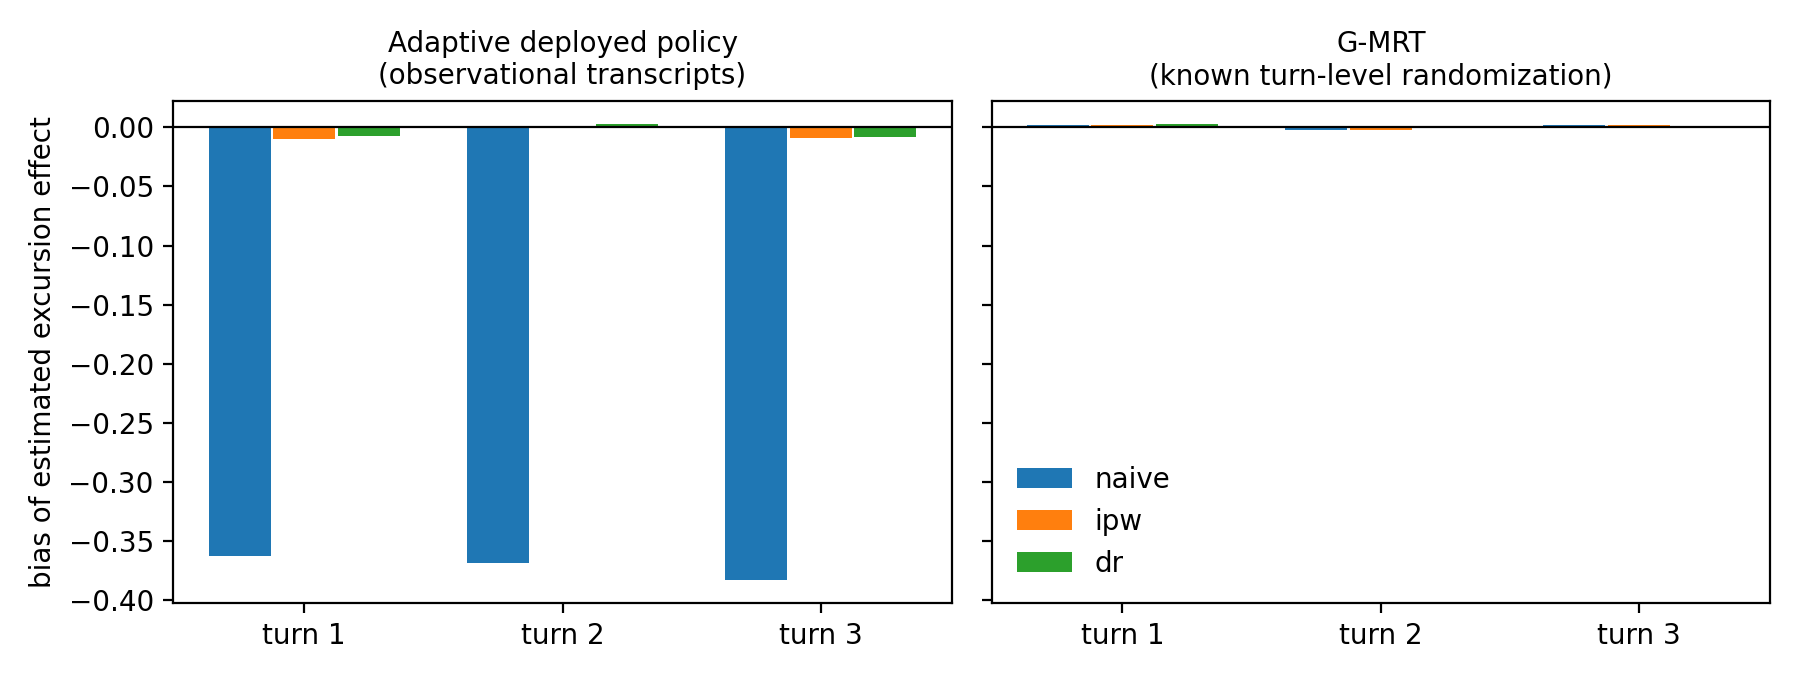
\includegraphics[width=0.8\textwidth]{figs/bias_plot.png}
\caption{Sign reversal under an adaptive policy: naive turn-level contrasts
versus known-$\rho$ IPW/DR.}
\label{fig:sign}
\end{figure}

\paragraph{(ii) Two-state temperature collapse.} Along a $\tau$ grid
calibrated so $\tau = 1$ reproduces the adaptive policy of (i): IPW SE grows
exponentially, tracking a scaled inverse-propensity diagnostic curve (labeled
as such --- it is not the efficiency bound); the naive estimator becomes
\emph{more confident while more wrong} as $\tau$ falls (coverage $\to 0$ with
shrinking SE) (Figure~\ref{fig:collapse}). Metric discipline: global
arm-specific Kish ESS (theory object), minimum stratum-arm cell occupancy
(rare-crossover diagnostic --- not Kish), $\E[p(1-p)]$ (Result~B object), and
$\E[2\min(p,1-p)]$ (diagnostic) are reported as four separate columns,
coverage both conditional and unconditional on estimability, with zero-cell
rates alongside. One finding we flag for practice: in the collapse regime the
\emph{realized} control-arm Kish ESS is non-monotone in $\tau$: it falls to
$0.028$ at $\tau = 0.40$, while the zero-stratum-arm rate is still $0.00$,
and then \emph{rebounds} to $0.037$, $0.372$, $0.534$ at $\tau = 0.30, 0.22,
0.15$ --- over exactly the range where the zero-stratum-arm rate climbs
$0.06 \to 0.70 \to 0.99$. Surviving
weights homogenize as rare crossovers vanish from the sample, so a
healthy-looking realized ESS co-occurring with high zero-cell rates is itself
the signature of the deceptive regime. ESS should never be reported without
zero-cell rates.

\begin{figure}[t]
\centering
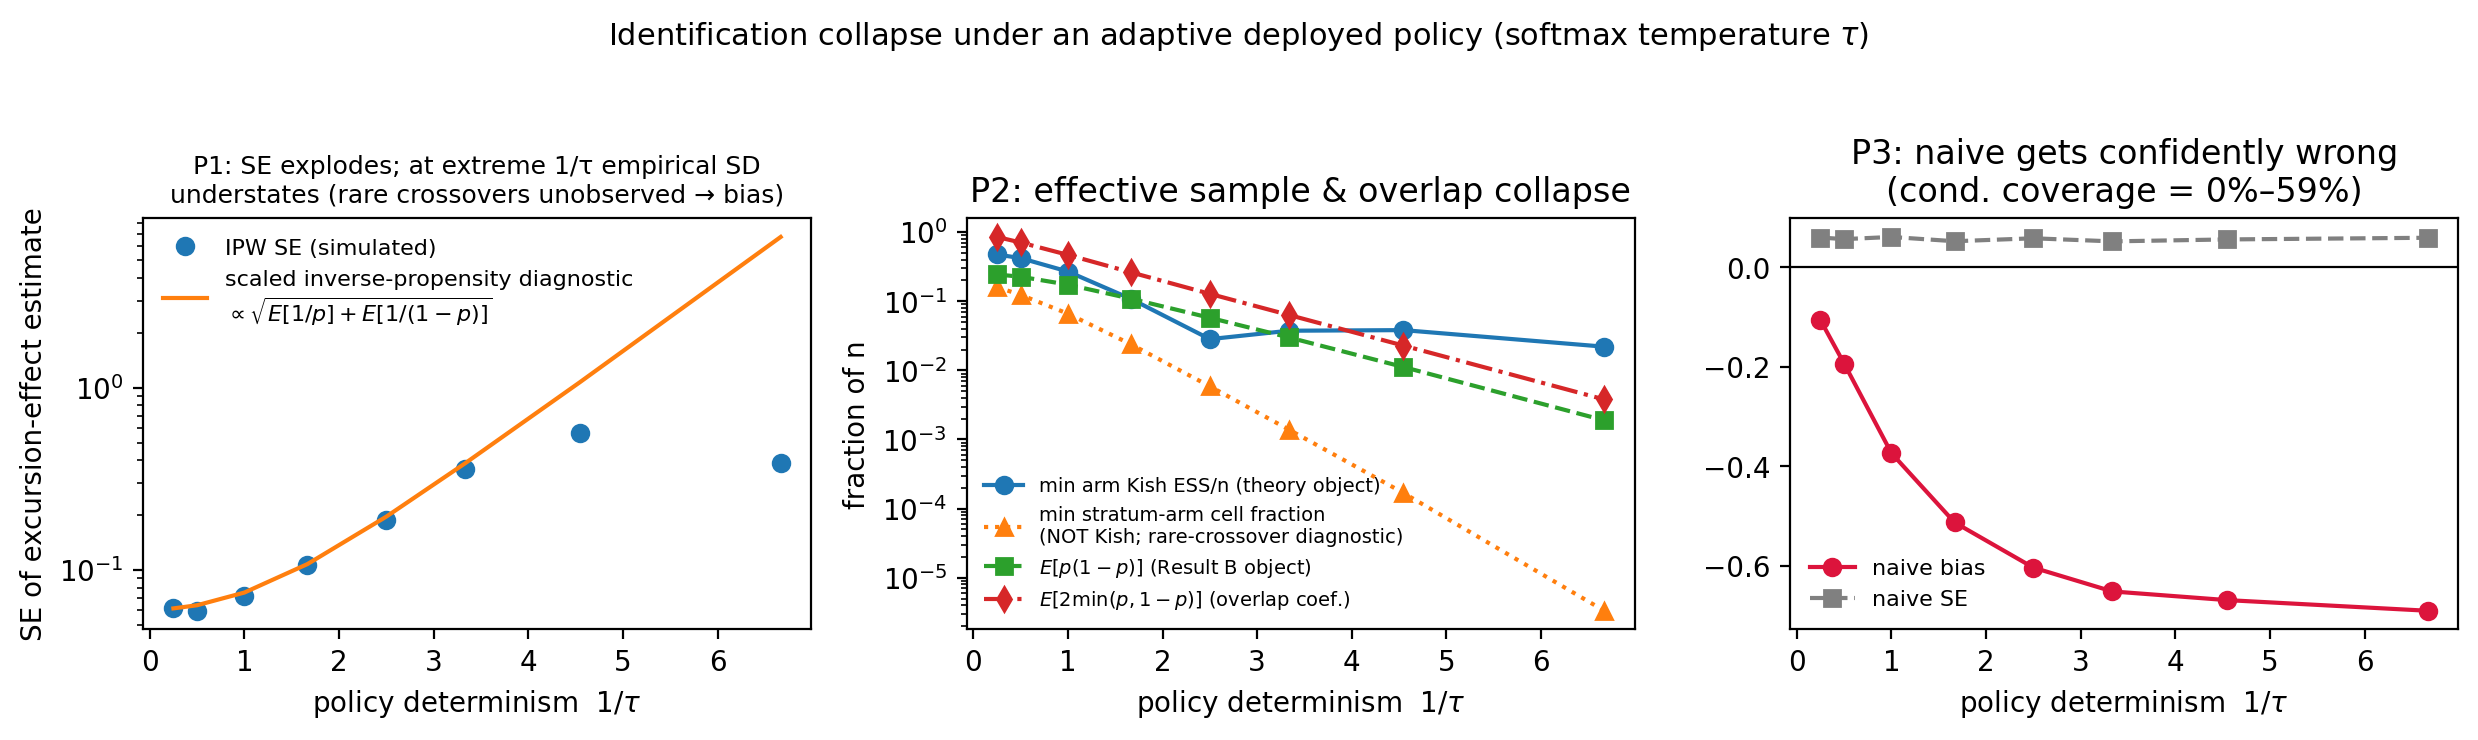
\includegraphics[width=\textwidth]{figs/collapse_curve.png}
\caption{Two-state temperature collapse: predictions P1--P3.}
\label{fig:collapse}
\end{figure}

\paragraph{(iii) Continuous-boundary battery.} ($H \sim U(-1,1)$ main,
$N(0,1)$ robustness; $\beta(H) \in \{1,\, 1+e^{-H^2},\, 1+|H|\}$; 400
replications per cell.) At $n = 32{,}000$: all population-targeting
estimators are unbiased with nominal coverage down to $\tau \approx 0.15$; at
$\tau = 0.045$ Horvitz--Thompson has SD 2.95 (variance explosion) while
H\'ajek shows bias 0.46 with SD 0.30 --- biased-yet-stable; oracle AIPW
retains nominal coverage throughout but does not rescue \emph{precision},
its SD inflating from 0.012 to 1.38 (a factor of 116) as $\tau$ falls ---
which is the behaviour Result~A predicts, and confirms that the efficiency
loss is not an IPW artifact; the oracle
outcome-regression line is flat by construction --- the (A3) escape made
visible, identification bought by assumption; and the overlap estimator
remains unbiased with nominal coverage \emph{for its own target
$\beta^{\ov}$} at every $\tau$, with $\beta^{\ov}_\tau \to \beta(0) = 1$ as
Result~B predicts (Figure~\ref{fig:battery}). Under $N(0,1)$ the collapse is
earlier and, at extreme $\tau$, propensities underflow to machine 0/1 so IPW
becomes numerically undefined --- reported as estimability 0, not dropped.

\begin{figure}[t]
\centering

\includegraphics[width=\textwidth]{figs/continuous_h_battery.png}
\caption{Estimator battery on the continuous-boundary design, $n = 4{,}000$
(bias against each estimator's own target; the overlap estimator targets
$\beta^{\ov}$). The numerical values quoted in the text are for $n =
32{,}000$, the largest cell of the grid.}
\label{fig:battery}
\end{figure}

\paragraph{(iv) Phase diagram.} The three regimes separate cleanly over the
$(n, \tau)$ grid (Figure~\ref{fig:phase}). We report the reference lines
without claiming either is the transition: measured onsets of estimability
lie $3$--$5$ nats above the $n_{\mathrm{eff}}=1$ contour, and on a widened
$13 \times 13$ grid neither a mean functional ($\log\E[e^{D}]$) nor an
upper-tail functional of $D$ reproduces a stable offset across the
$U(-1,1)$ and $N(0,1)$ designs. We therefore present the phase structure as
a simulation finding and leave its asymptotic characterization open.

\section{Empirical Plan and Ethics}\label{sec:plan}

The companion experimental paper implements the $2\times 2$ G-MRT: pilot $n =
80$--$120$ (function verification: assignment mechanics, fidelity rates, bank
leakage, dropout --- not effect detection), demonstration $n = 180$--$250$
with pre-registered minority contrasts, confirmatory sample from post-pilot
power simulation. Pre-registration locks the fidelity floor, blocking factors
(issue), attrition handling (IPW-for-attrition), and reactivity checks
(randomizing measurement itself in pilot). Ethics: persuasion toward
\emph{accuracy} on factual political questions with a fact-checked locked
bank \citep[cf.][]{costello2024durably}; no deception arms; disclosure of AI
interlocutor; IRB before pilot. The three Study 0 analyses involve only
public data and no new human subjects.

\section{Discussion}\label{sec:discussion}

What we rule in: estimand definitions that survive the generative setting;
explicit information limits with rates and locations; a design that restores
identification at a quantified exploration cost. What we rule out of this
paper: generator transport (effects across model versions --- motivated
empirically by cross-model heterogeneity in \citealp{chen2026benchmarking}),
internal-representation adjustment (overlap problems of representation
conditioning are themselves design-based cautionary tales,
cf.~\citealp{tierney2025design}), simultaneous inference over excursion
families, and epistemically constrained policy learning. Each is a
companion, not a section.

\paragraph{Limitations.} Five, stated plainly.

\emph{The bound is a constant, not a rate.} Proposition~\ref{prop:aprime}
bounds the asymptotic variance at a fixed policy. For any policy with
strictly positive action probabilities the excursion effect remains
regularly $\sqrt{n}$-estimable, and we do not prove that no estimator
escapes the \emph{rate}; that is a statement about drifting sequences and
requires a local asymptotic minimax argument we do not supply
(Remark~\ref{rem:notrate}).

\emph{We bound impossibility, not achievability.}
Proposition~\ref{prop:minimax} says when estimation must fail; it does not
say when it becomes easy, and the observed onset of estimability in
simulation is the latter. The two are separated by a design-dependent
amount: the gap between the lower-bound functional $M$ and the oracle-IPW
variance factor $\E[e^{D}]$ is $1.00$ nats for $U(-1,1)$ and $2.06$ for
$N(0,1)$. No single functional can therefore track both curves, and a
matching upper bound is left open.

\emph{Proposition~A-T rests on a recurrence condition in tension with our
own framing.} Condition (M1) requires histories to remain in the high-gap
set under \emph{every} action, i.e.\ that treatment does not move the
history state much --- which is close to the opposite of the premise in this
paper's title. Its per-turn factor is $\rho_{\min}^2 e^{D} p_\delta$, and
$p_\delta$ is not estimated anywhere here; multi-turn compounding should be
read as conditional on an unverified quantity.

\emph{Study~0 measures a projection, not a policy.} The entropy and
decisiveness figures in Section~\ref{sec:study0} are properties of an
eight-category strategy label assigned by an LLM judge, not of the
generation policy itself. Three specific threats: the modal category
(rebuttal) is near-tautological with the generation prompt, which asks for a
rebuttal; the two judges we ran agree at $\kappa = 0.13$ overall and not at
all once both-modal pairs are excluded, and the headline entropy figures
move materially between them; and at $k = 20$ regenerations a strategy with
true probability $0.02$ is unobserved with probability $0.67$, so
``never observed'' is not ``very rare.'' At the level of raw text the
generations are not degenerate at all --- within-context duplicates are
absent and pairwise lexical overlap is low. Any collapse we report is a
collapse \emph{after} projection to the label space. The re-queried models
are also open-weights stand-ins for the deployed system, not the deployed
system. We therefore use Study~0 to motivate and locate, not to establish;
human double-coding and higher-$k$ re-query on the censored subset are the
obvious next steps and are not yet done.

\emph{Study~0-c measures a bundled dose.} Realized fact counts covary with
AI verbosity ($r = 0.49$ and $0.71$ in studies 2 and 3), so the
within-assignment variance we report is not purely instruction--behavior
slippage; adjusting for message length \emph{raises} $\eta^2$ rather than
lowering it.

\paragraph{Data and code availability.} All numbers reported here are
produced by code in the project repository, which contains the simulation
sources, the analysis pipeline, the re-query outputs and judge labels, and
the derived result files. The DebateGPT reproduction uses the public
release of \citet{salvi2025conversational}; the deployment audit uses the
public release of \citet{hackenburg2025levers}, and the $56{,}831$
conversations are the released persuasion rows, not that paper's full
sample. Simulation entry points and expected runtimes are documented in the
repository README.

The one-sentence version of this paper: \emph{adaptive systems generate the
least population-level causal information exactly where they are most
decisive, and the information that survives lives on their decision
boundary} --- so if you want turn-level causal knowledge from conversational
AI, you must randomize the turns.

\appendix

\section{Efficient influence function and the decisiveness bound}
\label{app:eif}

\paragraph{Setup.} Observe $O = (H, A, Y)$ with $A \in \mathcal{A}$,
$|\mathcal{A}| = K < \infty$, and $\pi(a \mid h) = \Prob(A = a \mid H = h) >
0$ a.s. Write $\mu(a,h) = \E[Y \mid A=a, H=h]$ and $\sigma^2(a,h) = \Var(Y
\mid A=a, H=h)$; the model is nonparametric. In the multi-turn setting read
$H = H_t$, $Y$ as the proximal outcome, and all statements on the
availability stratum $\{I_t = 1\}$.

A regime is a known action distribution $q(\cdot \mid h)$ on $\mathcal{A}$
--- a stochastic intervention --- with value
$\psi(q) = \E\big[\sum_a q(a \mid H)\,\mu(a,H)\big]$. The form estimand of
Section~\ref{sec:framework} is $\beta^{\mathrm{form}} = \psi(q_1) -
\psi(q_0)$ with $q_1(f,d \mid h) = \mathbf{1}\{f = \text{assertive}\}
\rho_D(d)$ and $q_0$ likewise for interrogative. Note that the dose is
marginalized under the \emph{reference} $\rho_D$, not under $\pi$; this is
what makes the cell propensities, rather than the form-marginal, the
relevant quantities.

\begin{proposition}[Efficient influence function]\label{prop:eif}
$\psi(q)$ is pathwise differentiable with efficient influence function
\[
\varphi_q(O) \;=\; \sum_a q(a \mid H)\mu(a,H) \;-\; \psi(q) \;+\;
\frac{q(A \mid H)}{\pi(A \mid H)}\big(Y - \mu(A,H)\big),
\]
so that for $\beta = \psi(q_1) - \psi(q_0)$ the semiparametric efficiency
bound is
\begin{equation}\label{eq:E1}
V(\beta) \;=\; \Var\big(m_1(H) - m_0(H)\big) \;+\;
\E\Big[\textstyle\sum_a \big(q_1(a \mid H) - q_0(a \mid H)\big)^2
\frac{\sigma^2(a,H)}{\pi(a \mid H)}\Big],
\end{equation}
where $m_j(h) = \sum_a q_j(a \mid h)\mu(a,h)$.
\end{proposition}

\begin{proof}
$\psi(q)$ depends on the observed-data law only through the marginal of $H$
and the outcome regression $\mu$. Decompose the tangent space as
$\mathcal{T} = \mathcal{T}_H \oplus \mathcal{T}_{A \mid H} \oplus
\mathcal{T}_{Y \mid A,H}$ and differentiate along a regular parametric
submodel. The $\mathcal{T}_H$ component contributes $\sum_a q\mu - \psi$;
the $\mathcal{T}_{Y \mid A,H}$ component contributes $(q/\pi)(Y - \mu)$.
Because $q$ is a known function and $\psi$ does not depend on $\pi$, the
$\mathcal{T}_{A \mid H}$ component vanishes --- this holds even though $q$
may depend on $h$. One checks $\E[\varphi_q] = 0$ and $\varphi_q \in
\mathcal{T}$, so $\varphi_q$ is the EIF. The two components are orthogonal,
giving $\Var(\varphi_q) = \Var(m_q(H)) + \E[(q/\pi)^2\sigma^2]$; expanding
the second term over $a$ and using linearity in $q$ for the contrast yields
\eqref{eq:E1}.
\end{proof}

When $q_1$ and $q_0$ have disjoint support --- as they do for a form or
dose contrast --- $(q_1 - q_0)^2 = q_1^2 + q_0^2$ and the sum in
\eqref{eq:E1} runs over all $K$ cells.

\begin{definition}[Policy decisiveness]\label{def:D}
For $\mathcal{A}^* = \mathrm{supp}(q_1) \cup \mathrm{supp}(q_0)$ set
$D(h) := -\log \min_{a \in \mathcal{A}^*} \pi(a \mid h)$.
\end{definition}

$D$ is a functional of the behaviour policy alone and is identified from
logs; neither $\tau$ nor a softmax parameterization enters.

\begin{proposition}[Decisiveness bound; Result~A restated]\label{prop:aprime}
Assume (A1$'$) $\Prob\{D(H) \geq d\} \geq c > 0$; (A2$'$)
$\underline{\sigma}^2 := \inf\{\sigma^2(a,h) : D(h) \geq d,\ a \in
\mathcal{A}^*\} > 0$; and (A3). Let $\rho_{\min} = \min_{a \in
\mathcal{A}^*} q_j(a \mid h)$. Then
\[
V(\beta) \;\geq\; \underline{\sigma}^2 \rho_{\min}^2\,
\E\big[e^{D(H)}\big] \;\geq\; \underline{\sigma}^2 \rho_{\min}^2\, c\, e^{d}.
\]
\end{proposition}

\begin{proof}
Discard the first term of \eqref{eq:E1}. On $\{D \geq d\}$,
$\sum_a (q_1-q_0)^2 \sigma^2/\pi \geq \underline{\sigma}^2 \rho_{\min}^2
\sum_{a \in \mathcal{A}^*} 1/\pi(a \mid H) \geq \underline{\sigma}^2
\rho_{\min}^2 / \min_{a \in \mathcal{A}^*}\pi(a \mid H) =
\underline{\sigma}^2\rho_{\min}^2 e^{D(H)} \geq \underline{\sigma}^2
\rho_{\min}^2 e^{d}$; multiply by $\Prob\{D \geq d\} \geq c$.
\end{proof}

\begin{remark}[Recovering \citet{hahn1998role}]
With $K = 2$, $q_1 = \delta_1$, $q_0 = \delta_0$ (so $\rho_{\min} = 1$),
\eqref{eq:E1} is $\Var(\mu_1 - \mu_0) + \E[\sigma_1^2/\pi(1 \mid H) +
\sigma_0^2/\pi(0 \mid H)]$, i.e.\ the ATE bound of \citet{hahn1998role}. The
present paper therefore does not import that bound for a different estimand;
it derives the bound for the excursion estimand and recovers Hahn's as a
special case. If $\pi$ is a softmax at temperature $\tau$ and $K=2$, then
$D = |\Delta|/\tau + O(e^{-|\Delta|/\tau})$ and the $e^{\delta/\tau}$ form is
recovered; the converse fails, so Proposition~\ref{prop:aprime} applies to
sharply adaptive policies that are not softmax (truncated or constrained
decoding, learned $\arg\max$ rules, hard filters). For $K=2$ one also has the
exact identity $1/\{p(1-p)\} = 2 + 2\cosh(\mathrm{logit}\,p)$.
\end{remark}

\begin{remark}[Scope of Proposition~\ref{prop:aprime}]\label{rem:notrate}
The bound is a statement about the asymptotic variance at a \emph{fixed}
policy. Whenever $\pi(a \mid h) > 0$ everywhere, $V(\beta) < \infty$ and
$\beta$ remains regularly $\sqrt{n}$-estimable: on its own this is a
constant factor, not an impossibility. The impossibility statement requires
drifting sequences $\pi_n$ and is Proposition~\ref{prop:minimax} below; the
closest antecedent for the irregular behaviour it describes is
\citet{khan2010irregular}.
\end{remark}

\begin{proof}[Proof of Proposition~\ref{prop:minimax}]
Fix $d > 0$, let $\mathcal{H}_d = \{D \geq d\}$ and $c = \Prob(\mathcal{H}_d)
> 0$, and let $a^*$ attain the minimum in Definition~\ref{def:D}, so
$\pi(a^* \mid h) \leq e^{-d}$ on $\mathcal{H}_d$. Define two laws $P_0, P_1$
that agree in the marginal of $H$, in $\pi$, and in $\mu(a,h)$ for every
$(a,h)$ except one: $\mu^{(0)}(a^*,h) = 0$ and $\mu^{(1)}(a^*,h) =
\varepsilon$ for $h \in \mathcal{H}_d$.

\emph{Separation in the estimand.} Since $\psi(q) = \E[\sum_a q(a\mid H)
\mu(a,H)]$,
\[
\beta(P_1) - \beta(P_0) \;=\; \E\big[q(a^*\mid H)\,\varepsilon\,
\mathbf{1}\{H \in \mathcal{H}_d\}\big] \;\geq\; \rho_{\min}\,c\,\varepsilon
\;=:\; \Delta .
\]

\emph{Proximity in the data.} The observed density factorizes as
$P(H)\,\pi(A \mid H)\,N(Y; \mu_A(H), \sigma^2)$, and $P_0, P_1$ share the
first two factors, so only the $(a^*, \mathcal{H}_d)$ cell contributes to the
divergence:
\[
\mathrm{KL}(P_0 \| P_1) = \E_H\Big[\textstyle\sum_a \pi(a \mid H)\,
\mathrm{KL}\big(N(\mu^{(0)}_a,\sigma^2) \,\|\, N(\mu^{(1)}_a,\sigma^2)\big)
\Big] = c\,\pi(a^*\mid h)\,\frac{\varepsilon^2}{2\sigma^2}
\leq \frac{c\,e^{-d}\varepsilon^2}{2\sigma^2}.
\]
By tensorization $\mathrm{KL}(P_0^n \| P_1^n) = n\,\mathrm{KL}(P_0\|P_1)$.
Choose $\varepsilon = \sigma\sqrt{e^{d}/(nc)}$, so that this equals $1/2$;
Pinsker's inequality then gives $\mathrm{TV}(P_0^n, P_1^n) \leq
\sqrt{\mathrm{KL}/2} = 1/2$.

\emph{Le Cam.} The two-point bound
$\inf_{\hat\beta}\sup_P \E|\hat\beta - \beta| \geq (\Delta/2)(1 -
\mathrm{TV}) \geq \Delta/4$ with
$\Delta = \rho_{\min} c \varepsilon = \rho_{\min}\sigma\sqrt{c\,e^{d}/n}$.
Optimizing over $d$ replaces $c\,e^{d}$ by $M(\pi)$. The constraint
$|\mu| \leq B$ caps $\varepsilon$ at $B$, giving the stated minimum
\citep[for the two-point method see][\S2.2]{tsybakov2009introduction}. \qed
\end{proof}

\section{Support failure (Proposition~\ref{prop:1a})}\label{app:support}

Take $T=1$, $H \in \{h_0, h_1\}$ with $\Prob(H = h_1) > 0$,
$\pi^{\mathrm{dep}}(1 \mid h_0) = 1/2$ and $\pi^{\mathrm{dep}}(1 \mid h_1) =
0$, and $Y(a) \mid H=h \sim N(\mu_a(h), 1)$. Let two laws $P_1, P_2$ agree
in every component except $\mu_1(h_1)$, equal to $c_1$ under $P_1$ and $c_2
\neq c_1$ under $P_2$. The observed-data density factorizes as
$P(H)\,\pi^{\mathrm{dep}}(A \mid H)\,N(y; \mu_A(H), 1)$ and the stratum
$\{A = 1, H = h_1\}$ has probability zero, so $\mu_1(h_1)$ does not appear:
$P_1$ and $P_2$ induce identical observed-data laws. Their uniform-reference
excursion effects differ by $\Prob(h_1)(c_2 - c_1) \neq 0$. Hence no
functional of the observed-data law equals the excursion effect, which is
the claim. No latent confounder is used: the failure is support, not
confounding. The multi-turn version replaces $H$ by $(X, R_{1:t-1})$ and
recovers the standard time-varying-confounding form of
\citet{robins1986new}; the contribution here is not the structure but the
claim that the triggering condition is structurally frequent in RLHF-tuned
deployment, which is an empirical claim (Section~\ref{sec:study0}) and not a
theorem.

\section{Localization in one dimension (Proposition~\ref{prop:b})}
\label{app:resultB}

Throughout $\omega_\tau(h) = p_\tau(1-p_\tau) = \frac{1}{4}\mathrm{sech}^2
\!\big(\tfrac{\Delta(h)}{2\tau}\big) = \tfrac{1}{\tau}K\!\big(
\tfrac{\Delta(h)}{\tau}\big)$ with $K(u) = 1/[4\cosh^2(u/2)]$, an exact
identity. Two elementary facts: $\int_{\mathbb{R}} K = [\tfrac12
\tanh(u/2)]_{-\infty}^{\infty} = 1$, and $\cosh^2(u/2) \geq e^{|u|}/4$ gives
$K(u) \leq e^{-|u|}$.

Fix a bounded continuous $g$ and put $I_\tau(g) = \int \omega_\tau g f$.
Split at $U_\epsilon = \{\mathrm{dist}(h,\mathcal{R}) < \epsilon\}$. Outside
$U_\epsilon$, (B2$'$) gives $|\Delta| \geq \eta(\epsilon) > 0$, so
$\omega_\tau \leq e^{-\eta/\tau}$ and, $f$ and $g$ being bounded, that
contribution is $O(e^{-\eta/\tau}) = o(\tau)$. Inside, work near a single
root $r$ with $\Delta'(r) \neq 0$ (B2); by the inverse function theorem
$\Delta$ is a $C^1$ diffeomorphism of a neighbourhood of $r$ onto a
neighbourhood of $0$, so substituting $v = \Delta(h)$ and then $v = \tau u$,
\[
\int_{U_\epsilon} \omega_\tau g f \,dh
= \int K(u)\,\frac{(gf)(\Delta^{-1}(\tau u))}{|\Delta'(\Delta^{-1}(\tau u))|}
\,\tau \,du .
\]
The integrand is dominated by $K(u)\sup_{|h-r| \leq \epsilon}
|gf/\Delta'|$, finite because $|\Delta'|$ is continuous and bounded away
from $0$ near $r$; by dominated convergence and continuity of $f$, $g$ at
$r$ the integral tends to $g(r)f(r)/|\Delta'(r)|$. Hence
$I_\tau(g) = \tau\,g(r)f(r)/|\Delta'(r)| + o(\tau)$. Summing over the
finitely many roots (B2) gives $I_\tau(g) = \tau \sum_j
g(r_j)f(r_j)/|\Delta'(r_j)| + o(\tau)$. Taking $g \equiv 1$ yields the
statement for $\E[\omega_\tau]$, where (B4) $f(r) > 0$ for some root is
exactly what prevents the leading term from vanishing and the expansion
from degenerating to $0 = o(\tau)$. Ratios $I_\tau(g)/I_\tau(1)$ give weak
convergence to $\sum_j w_j \delta_{r_j}$ with $w_j \propto
f(r_j)/|\Delta'(r_j)|$, and $g = c$ (bounded, continuous near the roots, by
(B3)) gives the limit of $\beta^{\ov}_\tau$. With a unique root at $0$ this
is a point mass and $\beta^{\ov}_\tau \to c(0)$. \hfill$\square$

\section{Localization on a decision manifold (Corollary~\ref{cor:manifold})}
\label{app:manifold}

Let $H \in \mathbb{R}^d$ and $\mathcal{B} = \Delta^{-1}(0)$. By (C2),
$\nabla\Delta \neq 0$ on $\mathcal{B}$, so $0$ is a regular value and
$\mathcal{B}$ is a $C^1$ hypersurface of dimension $d-1$. On $U_{\epsilon_0}
= \{|\Delta| < \epsilon_0\}$ the coarea formula (e.g.\ Evans and Gariepy,
Thm.\ 3.4.2) gives, for integrable $\Phi$,
\[
\int_{U_{\epsilon_0}} \Phi \,dh
= \int_{\mathbb{R}} \Big[ \int_{\Delta^{-1}(s)}
\frac{\Phi}{\|\nabla\Delta\|}\,d\mathcal{H}^{d-1}\Big] ds .
\]
Apply this with $\Phi = \omega_\tau g f$. Since $\omega_\tau$ depends on $h$
only through $\Delta(h)$, it is constant on level sets and factors out:
with $G(s) := \int_{\Delta^{-1}(s)} gf/\|\nabla\Delta\|
\,d\mathcal{H}^{d-1}$,
\[
\int_{U_{\epsilon_0}} \omega_\tau g f \,dh
= \int_{-\epsilon_0}^{\epsilon_0} \tfrac{1}{\tau}K(s/\tau)\,G(s)\,ds
= \int_{|u| \leq \epsilon_0/\tau} K(u)\,G(\tau u)\,du \cdot \tau .
\]
By (C1)--(C2) and the implicit function theorem the level sets
$\Delta^{-1}(s)$ vary continuously in $s$ near $0$ along the normal flow of
$\mathcal{B}$, and $f$, $g$, $\|\nabla\Delta\|$ are continuous with
$\|\nabla\Delta\|$ bounded away from $0$; hence $G$ is continuous at $0$
with $G(0) = \int_{\mathcal{B}} gf/\|\nabla\Delta\| \,d\mathcal{H}^{d-1}$.
Since $\int K = 1$ and $K(u) \leq e^{-|u|}$, dominated convergence gives
$\int_{U_{\epsilon_0}} \omega_\tau g f = \tau\,G(0)\,(1 + o(1))$. The region
outside $U_{\epsilon_0}$ contributes $O(e^{-\eta/\tau})$ by (C4) as in
Appendix~\ref{app:resultB}. Taking $g \equiv 1$ gives the stated expansion
of $\E[\omega_\tau]$; (C5) guarantees the limit is in $(0,\infty)$, so
ratios converge and the normalized overlap measure tends weakly to the
measure on $\mathcal{B}$ with $\mathcal{H}^{d-1}$-density proportional to
$f/\|\nabla\Delta\|$. Taking $g = c$ gives the limit of $\beta^{\ov}_\tau$.
For $d = 1$, $\mathcal{H}^0$ is counting measure and $\|\nabla\Delta\| =
|\Delta'|$, recovering Appendix~\ref{app:resultB}. \hfill$\square$

\bibliographystyle{plainnat}
\bibliography{../references}

\end{document}
